\section{Fluid Mechanics}
\subsection{Kinematics}
\subsubsection{Coordinates}
\textbf{Lagrangian} $\underline{\boldmath{x}}(\underline{\boldmath{a}},t)$: The \textit{motion of individual particles} is studied; the position $\underline{\boldmath{x}}$ of a particle at time $t$ is related to its position at a reference point in time \underline{\boldmath{a}} (typically at $t=0$).
\newline
\newline
\textbf{Eulerian} $(\underline{\boldmath{x}},t)$: 
The \textit{'flow field' is considered as a whole} and the state of a fluid is described in terms of the values at a fixed location $\underline{\boldmath{x}}$ and at fixed time $t$
\subsubsection{Velocity}
In Cartesian coordinates the velocity of a fluid particle at position $\underline{\boldmath{x}}(x,y,z)$ is given by:
\begin{center}
	$\underline{\boldmath{u}}(x,y,z) = u(x,y,z)\underline{\hat{i}} + v(x,y,z)\underline{\hat{j}} + w(x,y,z)\underline{\hat{k}}$
\end{center}
\subsubsection{Stagnation Points}
Stagnation points occur when the velocity vector $\underline{u}$ is equal to $\underline{0}$
\begin{align*}
	u = 0
	\\
	v= 0
	\\
	w= 0
\end{align*}
\subsubsection{Streamlines}
A streamline is a curve $C$ drawn at one point in time such that the fluid velocity vector $\underline{u}$ is tangent to $C$ at every point along $C$.
\begin{center}
	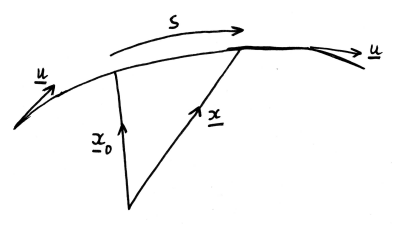
\includegraphics[width = 0.5\textwidth]{"Images/Streamline.png"}
\end{center} 
\begin{align*}
	\frac{d\underline{x}}{ds} = \underline{u}
	\\
	\\
	\frac{dx}{ds}=u , \frac{dy}{ds}=v ,  \frac{dz}{ds}=w
	\\
	\\
	\boxed{\frac{dx}{u}=\frac{dy}{v}=\frac{dz}{w}(= ds)}
\end{align*}

\subsubsection{Particle Paths}
Particle path is obtained by solving the initial value problem:
\begin{center}
		$\frac{d\underline{x}}{dt} = \underline{u}(\underline{x},t)$ , $\underline{x} = x_0$ at $t = 0$
		\\
		\begin{tabular}{|c|}
			\hline
			\\
				$\frac{dx}{dt} = u$ , $x(0)=x_0$
			\\ 
			\\
			$\frac{dy}{dt} = v$, $y(0)=y_0$
			\\
			\\
			$\frac{dz}{dt} = w$, $z(0)=z_0$
			\\
			\\
			\hline
		\end{tabular}
\end{center}

	
		


\subsubsection{Steady Flow}

\textbf{Steady Flow}: The flow velocity vector $\underline{u}$ is independent of time $t$
\newline
\textbf{Unsteady Flow}: $\underline{u}$ depends on $t$; the pattern of streamlines changes with $t$
\subsubsection{Convective Derivative}
The convective derivative tells us how a property changes \textit{as it moves with a flow}.

\subsubsection{Vorticity}

\subsection{Pressure in a Fluid}
\subsection{Flow Dynamics}
\subsection{Tow-dimensional Flow}
\subsection{Vorticity Dynamics}
\subsection{Free Surface Waves}